% id: 113-03
% book: 베이직쎈 확률과 통계 · 06 이항분포와 정규분포
% section: 유형 066 정규분포곡선의 성질
% figure: tikz:fig-113-03
% answer: 
% answer_source: 
% variant_level: 0 (원본 전사)
% 이 파일은 build.mjs 가 items.json 에서 만든다. 고칠 때는 items.json 을 고친다.
\smash{\raisebox{1.5mm}{\dmkichul{베이직쎈 확률과 통계 113쪽 03번}}}
\noindent\begin{minipage}[t]{0.58\linewidth}\vspace{0pt}\raggedright 학생 수가 서로 같은 두 고등학교 $\mathrm{A}$, $\mathrm{B}$의 학생들의 영어 점수를 각각 $X_{\mathrm{A}}$, $X_{\mathrm{B}}$라 할 때, 두 확률변수 $X_{\mathrm{A}}$, $X_{\mathrm{B}}$는 정규분포 $\mathrm{N}(m_{\mathrm{A}}{,}\mkern3mu\mathopen{}{\sigma_{\mathrm{A}}}^2)$, $\mathrm{N}(m_{\mathrm{B}}{,}\mkern3mu\mathopen{}{\sigma_{\mathrm{B}}}^2)$을 따른다. 위의 그림의 두 곡선 $\mathrm{A}$, $\mathrm{B}$는 각각 $X_{\mathrm{A}}$, $X_{\mathrm{B}}$의 확률밀도함수의 그래프일 때, 옳은 것만을 \textbf{보기}에서 있는 대로 고르시오. \end{minipage}\hfill\begin{minipage}[t]{0.4\linewidth}\vspace{0pt}\centering \resizebox{\ifdim\width>\linewidth\linewidth\else\width\fi}{!}{% 113-03(인쇄 113쪽) — 유형 066 03번의 두 정규분포곡선 A, B(A 는 왼쪽·높고 좁게, B 는 오른쪽·낮고 넓게 · 대칭축 점선 없음).
% 스캔 화질이 낮아 TikZ 로 다시 그림. 라벨은 원문에 있는 것만(A, B, x)이고 평균·표준편차의 값은 적지 않는다.
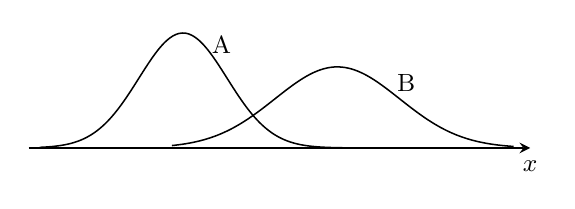
\begin{tikzpicture}[x=0.70cm, y=1.05cm, line width=0.55pt, font=\small]
  \draw[->, >=stealth, line width=0.7pt] (-4.3,0) -- (4.8,0) node[below=1pt] {$x$};
  \draw plot[domain=-4.1:1.6, samples=100, smooth] ({\x},{1.39*exp(-(\x+1.5)*(\x+1.5)/(2*0.80*0.80))});
  \draw plot[domain=-1.7:4.5, samples=100, smooth] ({\x},{0.98*exp(-(\x-1.3)*(\x-1.3)/(2*1.13*1.13))});
  \node at (-0.80,1.24) {$\mathrm{A}$};
  \node at (2.55,0.78) {$\mathrm{B}$};
\end{tikzpicture}
}\end{minipage}\par
\noindent \bogi{ㄱ. $\mathrm{P}(X_{\mathrm{A}}\ge m_{\mathrm{A}})=\mathrm{P}(X_{\mathrm{B}}\ge m_{\mathrm{B}})$\\ ㄴ. $\mathrm{A}$ 고등학교 학생들의 영어 점수의 평균이 $\mathrm{B}$ 고등학교 학생들의 영어 점수의 평균보다 높다.\\ ㄷ. $\mathrm{B}$ 고등학교 학생들의 영어 점수가 $\mathrm{A}$ 고등학교 학생들의 영어 점수보다 더 고르다.}
